\documentclass[12pt]{article}
\setlength\parindent{0pt}
\usepackage{fullpage}
\usepackage{amsmath}
\usepackage{graphicx}
\usepackage{enumitem}
\setlength{\parskip}{4mm}
%\usepackage[left=2cm, right=2cm, top=1.5cm, bottom=1cm]{geometry}
\usepackage[margin=0.5in, paperwidth=13.5in, paperheight=8.4375in]{geometry}
\def\LL{\left\langle}   % left angle bracket
\def\RR{\right\rangle}  % right angle bracket
\def\LP{\left(}         % left parenthesis
\def\RP{\right)}        % right parenthesis
\def\LB{\left\{}        % left curly bracket
\def\RB{\right\}}       % right curly bracket
\def\PAR#1#2{ {{\partial #1}\over{\partial #2}} }
\def\PARTWO#1#2{ {{\partial^2 #1}\over{\partial #2}^2} }
\def\PARTWOMIX#1#2#3{ {{\partial^2 #1}\over{\partial #2 \partial #3}} }
\newcommand{\BI}{\begin{itemize}}
\newcommand{\EI}{\end{itemize}}
\newcommand{\BE}{\begin{displaymath}}
\newcommand{\EE}{\end{displaymath}}
\newcommand{\BNE}{\begin{equation}}
\newcommand{\ENE}{\end{equation}}
\newcommand{\BEA}{\begin{eqnarray}}
\newcommand{\EEA}{\nonumber\end{eqnarray}}
\newcommand{\EL}{\nonumber\\}
\newcommand{\la}[1]{\label{#1}}
\newcommand{\ie}{{\em i.e.\ }}
\newcommand{\eg}{{\em e.\,g.\ }}
\newcommand{\cf}{cf.\ }
\newcommand{\etc}{etc.\ }
\newcommand{\Tr}{{\rm tr}}
\newcommand{\etal}{{\it et al.}}
\newcommand{\OL}[1]{\overline{#1}\ } % overline
\newcommand{\OLL}[1]{\overline{\overline{#1}}\ } % double overline
\newcommand{\OON}{\frac{1}{N}} % "one over N"
\newcommand{\OOX}[1]{\frac{1}{#1}} % "one over X"

\def\BS{\bigskip}

\begin{document}
\pagenumbering{gobble}
\Large
\centerline{\sc{Recitation Questions -- Vectors}}
\normalsize
\centerline{\sc{18 February}}

\it Your assessment for this recitation will be a brief question about the homework that you turned in today. You may discuss it with your group, but each person should answer individually. There will be a Blackboard quiz that ``goes live'' ten minutes before the end of the recitation period. Five minutes before the end of the recitation period, you should stop what you are doing and answer the question on Blackboard.

\rmfamily

\medskip

\rm In this recitation, you will practice:

\BI
\item Converting vectors from ``magnitude and direction'' representation to ``$x-$ and $y-$component'' representation
\item Breaking vectors into their $x-$ and $y-$ components
\item Representing vectors in different coordinate systems
\item Using vector addition and subtraction to solve problems
\EI
\newpage
\begin{minipage}{0.45\textwidth}
{\bf Question 1.} The streets in Manhattan are laid out in a grid, but that grid is aligned with the island, rather than along the compass directions. Avenues run 28.9 degrees east of north, while streets run 28.9 degrees north of west. 

This means that there are two sensible coordinate systems in Manhattan:

\BI
\item North/South/East/West, aligned with the compass
\item Uptown/Downtown/Crosstown, aligned with the streets.
\EI


\BS\BS

The staff astronomer at the Natural History Museum walks from Penn Station to the Natural History Museum, going 3.3 km north along Eighth Avenue. How far east and how far north did she walk? ({\it Note: Her path carries her off of the top of the page. You will want to draw an arrow aligned with her path below, and then draw its components.})

\vspace{3in}

\end{minipage}
\hspace{0.05\textwidth}
\begin{minipage}{0.48\textwidth}
	
	\begin{center}


	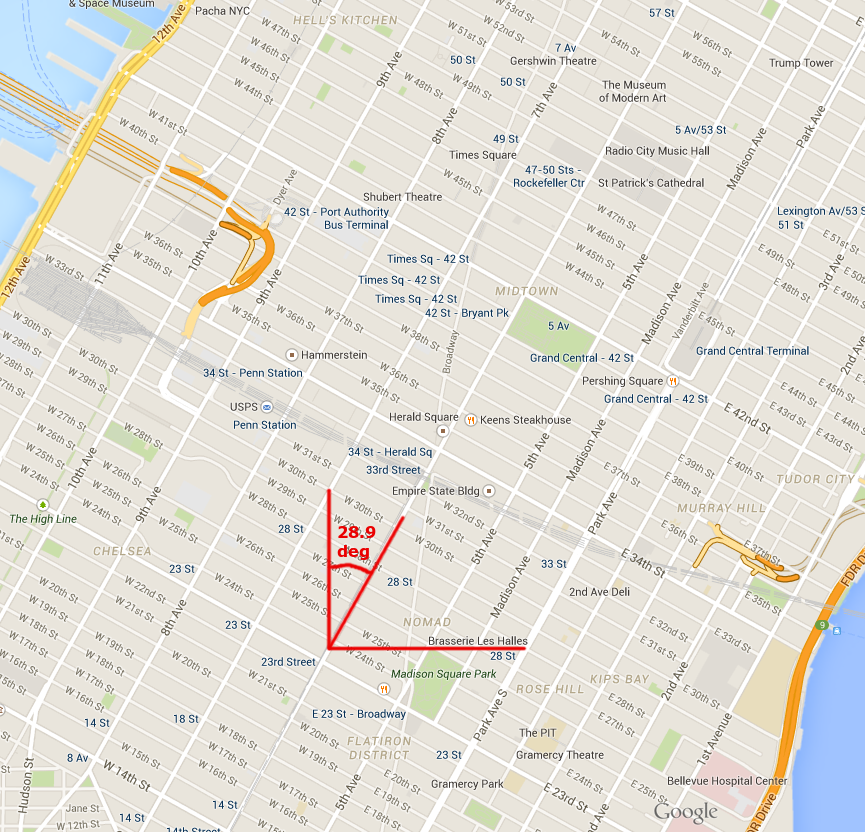
\includegraphics[width=\textwidth]{manhattan-1.png}
	
	(In this map and the next one, “up” is due north.)
	\end{center}
\end{minipage}

\newpage

\begin{minipage}{0.45\textwidth}
{\bf Question 2.} Here is the displacement vector pointing from the Metropolitan Opera to Carnegie Hall.
	\BS
	
	Draw on top of the picture on the right:
	
	\BI
	\item its component in the direction of the Manhattan avenues;
	\item its component perpendicular to them;
	\item its component along the North-South axis;
	\item its component along the East-West axis.
	\EI

	
	It may be helpful to draw the first two on the bottom and left in one color, and the second two on the top and right in a different color.
	\vspace{1in}
	\vspace{3in}	
\end{minipage}
\hspace{0.05\textwidth}
\begin{minipage}{0.48\textwidth}
	
	\begin{center}
		
		
		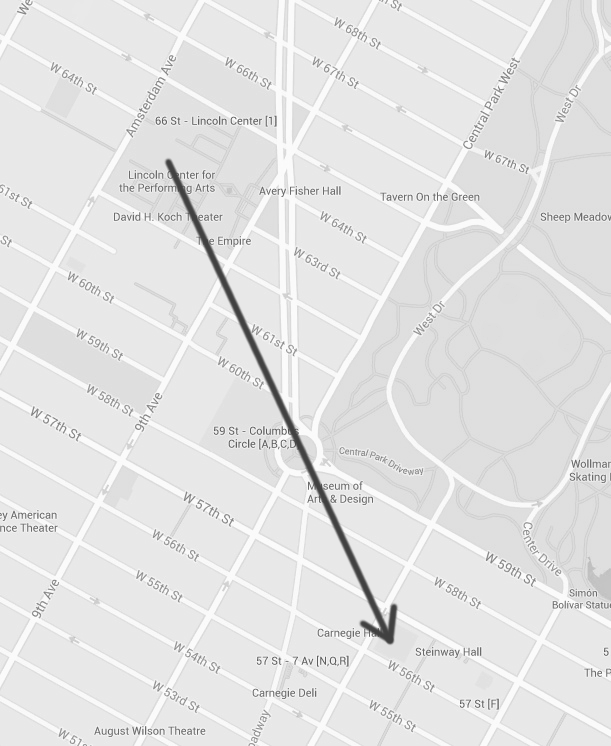
\includegraphics[width=\textwidth]{manhattan-2.png}
		
	
	\end{center}
\end{minipage}
\newpage
{\bf Question 3.}A hiker in the forest walks 5 km due north and then 2 km due east, and then wants to return to his original spot by the shortest route possible. 

Draw the hiker's path. 








\vspace{3in}

Which direction should he walk, and for how far?










\newpage
{\bf Question 4.} Now our hiker walks 3 km due north, then 4 km at an angle 30 degrees south of east, and then finally 5 km at an angle 45 degrees north of west. He then wants to return to his starting point, as before. Which direction should he travel in, and for how far? 

Hint 1: It will help visualize things to draw the hiker's path first.

Hint 2: Remember that you can add vectors by converting them to $x-$ and $y-$components and then adding the components. The simplest approach here is:

\begin{enumerate}
	\item Convert the vectors to component form
	\item Add the components
	\item Convert the resulting sum back to the magnitude-and-direction form that you are looking for.
\end{enumerate}

\newpage
{\bf Question 5.} A swimmer can swim 5 km/hr in still water. She wants to swim directly across a river. However, there is a current in the river, with a speed of 2 km/hr. If she swims directly across, she will drift downstream due to the current. Thus, in order to get where she wants to go, she needs to angle herself upstream.

\begin{enumerate}
\item There are three interesting vectors in this problem: the velocity of the current, her velocity relative to the current, and her velocity relative to the shore. How do they relate? State this both mathematically (for instance, “this vector plus that vector equals this other vector”), and geometrically (draw a picture).
\vspace{3in}











\item At what angle must she try to swim in order to proceed directly across the river?





\vspace{1.5in}




\item If the river is 200 m across, how long will it take her to cross?

\end{enumerate}




\end{document}
